
\section{Summative Evaluation}
\label{sec:summative-evaluation}

Phase~D of the project
%  (June 2011 February 2012, see Section~\ref{sec:methodology}) 
included summative evaluation of the TA tools,
comprised of two parts. 

The first part of the summative evaluation was a
classroom-based trial involving one of our teacher collaborators at
her school. This teacher had worked closely with us in Phase A and
was one of the two teachers who had participated in a classroom
trial in Phase B. A one-to-one discussion was first held with this
teacher where she was introduced to the final versions of the TA
tools and where she planned two one-hour lessons that she would
undertake with a class of 28 14-year-olds using the MiGen system.
During the first lesson, the TA tools were installed on a tablet PC
which she carried around the class with her and consulted as she
wished as her students were undertaking the task set in
eXpresser. During the second lesson, which took place the next day,
the teacher did not have access to the TA tools and had to support the
students as they were working with eXpresser without having access to
the information that the TA tools provide. The
aim of this second lesson was to compare the difference in the
teacher's experience compared to the first lesson in which she could
access the TA tools.

During and at the end of both lessons, the teacher was
asked a number of questions by a member of the research team, 
covering between them all the usage scenarios US1--US8, 
with the aim of evaluating the extent to which the TA tools 
meet the requirements of the usage scenarios. 
The questions are listed in Figure~\ref{fig:summquest}. 
A key objective when formulating and posing these questions 
was to disrupt the interaction between teacher and students as little as possible: 
we wished to introduce minimal additional cognitive load 
on the teacher, aiming for questions that could be answered quickly
and yet precisely; 
also, we wished to impact as little as possible on the teacher's role
in monitoring students' progress and in supporting students in
completing the task set. 

All the questions were designed to be
answerable in less than 60 seconds. 
They were not asked if the teacher was helping 
a student, only when the teacher was moving around the class. 
The teacher was interrupted only three times during the lesson, each time for no more
than 60 seconds, and was asked the questions at approximately the times shown in
Figure~\ref{fig:summquest}. 
Additional questions were posed during a debriefing session
after the end of each lesson.

\begin{figure}[hbtp]
  Question 1 (15 minutes into the lesson): which students are
  progressing satisfactorily in undertaking the task? [relates to
  Usage Scenario US2], which students may be in difficulty?
  [US2], which students need your immediate help? [US1]

  Question 2 (at 25 minutes): which students may be disengaged from the task?
  [US3], which students have achieved Task Goal 3? [US6]

  Question 3 (at 35 minutes): what common conceptual or procedural
  difficulties are students facing? [US4], what explanation might you
  give to the whole class at this time? [US4]

  Question 4 (at the end of lesson): now that the lesson has finished,
  (i) which students have finished the task? [US5], 
  (ii) what additional guidance might you give to any particular students? [US7].

  Question 5 (after end of lesson): what are your views about the
  class' achievements in this lesson? how might you plan the next
  lesson? [US8]

  \caption{Questions asked to the teacher during and after the lessons}
  \label{fig:summquest}
\end{figure}

 

In the first lesson --- using the TA tools --- the
teacher was able to answer quickly and effectively Question~1 and
Question~2. For example, when asked ``which students have achieved Task
Goal~3?'' she correctly selected the GA tool and
pointed to the students who were being shown (in green) as achieving
that goal. At the end of the lesson, the teacher answered correctly
Question~4(i). 
%
During the debriefing, the teacher said that
answering Questions 3 and 4(ii) required having a global view of the
class' `learning status' which was difficult to obtain from the tools (even
more so, of course, without them).
% 
% This points to future work on HLI.
%
Regarding Question~5, she commented on her plans for the next lesson
using the information provided by the tools to ground her arguments, e.g.~``I
see that there are several students that did not complete the last
goal (general rule), so I will make a stronger point about it [next
day] to make it clearer''. 


On the second day --- without the TA tools --- the teacher was able to
answer the questions only in vague terms, e.g.~``I think one of
those students over there has finished''. In the after-lesson debriefing,
she commented that having access to the TA tools during the first lesson 
had made a real difference and that without them it was infeasible to 
obtain a ``view'' of the class, because
paying attention to so many students required very frequent changes of
context and ``the forest gets lost behind the trees''. 



The second part of the summative evaluation involved a 2-hour session
held with a new cohort of 11 trainee Maths teachers on the
Postgraduate Certificate in Education programme at the Institute of Education. 
Each of the participants had an installation of the MiGen system running on
their computer. In the first half of the session, participants were
introduced to the MiGen system as a whole, the
eXpresser, and the TA tools. In particular, the TA tools were
introduced to participants loaded with the real student interaction
data as arising from the classroom trials undertaken in the first part
of the summative evaluation and described above. Participants were
asked to use the TA tools and the time-stop functionality to
answer a short list of questions relating to usage scenarios US1-US6
at different time points in the lesson, simulating in this
way the use of the tools in a real classroom.
The questions are listed in Table~\ref{fig:questions-pgce}. 
Participants were also asked how long they thought it would take them to
answer these questions in a lesson
(selected from 1 -- Very little time,
2 -- A little time,
3 -- Average time, 
4 -- A long time, 
5 -- A lot of time),
our aim being not only to
determine if participants were able to use the TA tools to answer the
questions correctly, but also how they perceived the amount of time that it
would take them to answer the questions in a classroom situation. 

\begin{table}[tb]
  \centering
  \begin{framed}
  \begin{itemize}
  \item Q1. The session started 10 minutes ago (10 minutes into the lesson). 
    If you chose a student to help immediately, 
    which student(s) would you choose and why?
  \item Q2. Based on your experience and previous sessions you would have
    expected by now (10 minutes on) that students have achieved at
    least two goals. With a quick glance of the tools would you say
    that the class overall is going according to plan or would you
    intervene and why?
  \item Q3. We are at 30 minutes on. Based on your experience and
    previous sessions you expected that students would have finished
    by now so that you can progress on the next task. With a quick
    glance of the tools do you think that the class is at that stage
    and why?
  \item Q4. Sometimes students are off-task (e.g. play
    games). A 30 minutes on, find two students that are
    disengaged/distracted. 
  \item Q5. We are at 30 minutes. Some students need help and you are
    trying to identify others who have finished and can help them. Can
    you give two examples of students who have finished? 
  \end{itemize}    
  \end{framed}
  \vspace{-1em}
  \caption{Questions asked to trainee Maths teachers for summative
    evaluation of the TA tools. Teachers were asked to answer each
    question and also record the time they needed to do so.} 
  \label{fig:questions-pgce}
\end{table}

All participants provided correct answers without any assistance from the
research team. The graph shown in Figure~\ref{fig:perceived-time}
summarises the responses relating to the perceived length of time required to
answer each question. We see that for all
the questions no participant responded ``A long time'' or 
``A lot of time''. 
The questions regarded as
requiring the least time to answer were Questions 1, 4 and 5, 
most probably because they pertain to individual students and could be
answered by consulting just one tool (the CD tool). Questions 2
and 3 may have appeared to participants as taking more time to answer
because they refer to the classroom as a whole and because, in order
to answer them, participants may have consulted the GA tool
as well, and even the ST tool in Question 2 for a more detailed view
of how students are progressing with their constructions. 

% On the
% whole, we consider the responses satisfactory particularly as no
% answers were perceived as requiring long or a lot of time, which was
% our aim. 

\begin{figure}[htbp]
  \centering
    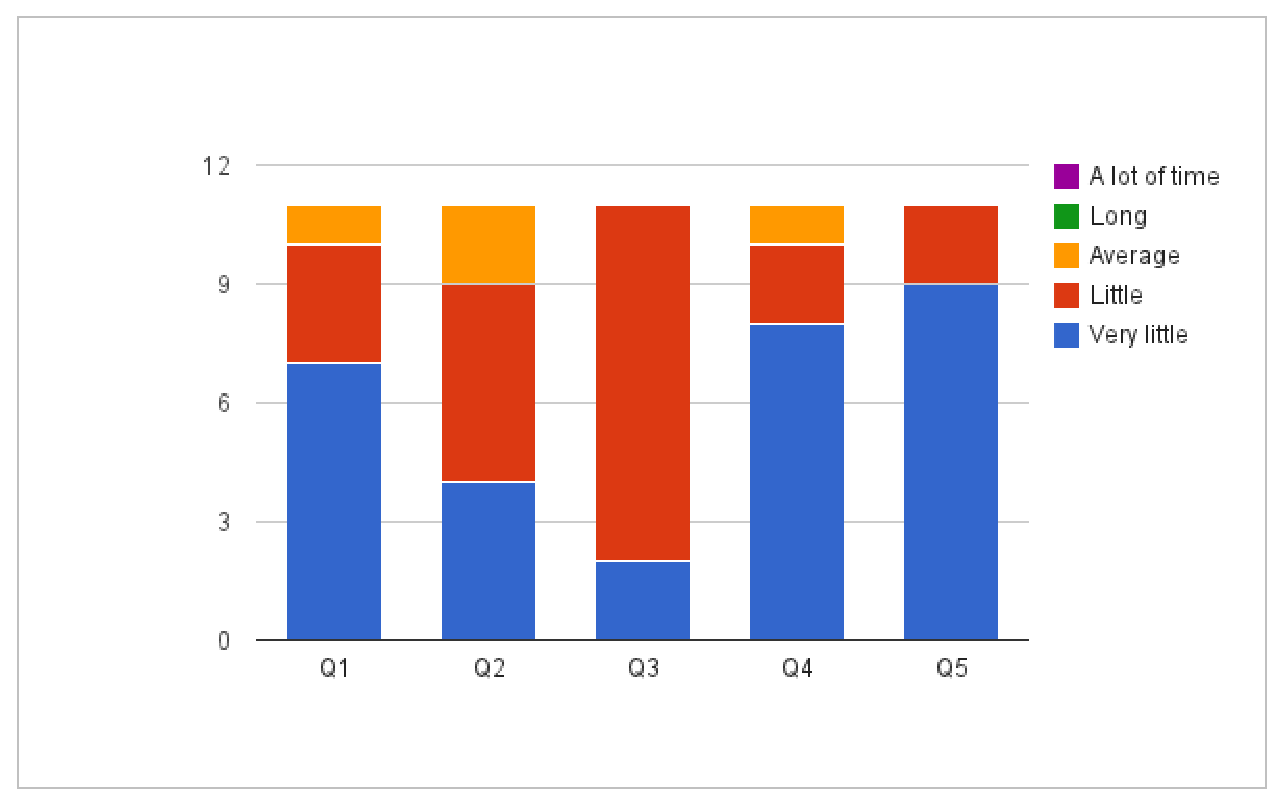
\includegraphics[width=\textwidth]{gfx/perceived-time-Q1-Q5.eps}
  \caption{Participants' perceived time to answer the questions in
Table~\ref{fig:questions-pgce}} 
\label{fig:perceived-time}
\end{figure}


Finally, at the end of the session, 
participants were asked to respond to the list of
questions in Figure~\ref{fig:questions2-pgce}, 
relating to their perceived usefulness of the TA tools for
the usage scenarios US1--US8. Question 1 relates to US1, Question 2 to US3, 
Question 3 to US6, Question 4 to US2 and US7(i), Question 5 to US7(ii), 
Question 6 to US8, and Question 7 to US4. Their
response to each question was selected from: 1 -- Totally Agree,
2 -- Agree, 3 -- Not sure, 4 -- Disagree, 5 -- Totally Disagree.

\begin{figure}[htbp]
  \begin{framed}
  I think that the Teacher Assistance Tools can help me\ldots
  \begin{enumerate}
  \item \ldots in the
    classroom to find out which students need the teacher's immediate
    help.
  \item \ldots in the classroom to find out which students are
    currently disengaged from the task or distracted.
  \item \ldots to identify which goals have been achieved by which
    students.
  \item \ldots to provide appropriate support and guidance to individual
    students during the lesson.
  \item \ldots to provide appropriate support and guidance to individual
    students and reflect on the class' progress after the lesson.
  \item \ldots to reflect on the class' achievements and to plan for
    the next lesson.
  \item either in the classroom or after the class, to identify common
    conceptual and procedural difficulties students are facing in
    order to prove more explanation to the class as a whole in the
    current or the next session.
  \end{enumerate}
  \end{framed}
  \vspace{-1em}
  \caption{Additional questions asked to trainee Maths teachers for 
    summative evaluation of the TA tools.} 
  \label{fig:questions2-pgce}    
\end{figure}



\begin{figure}[htbp]
  \centering
    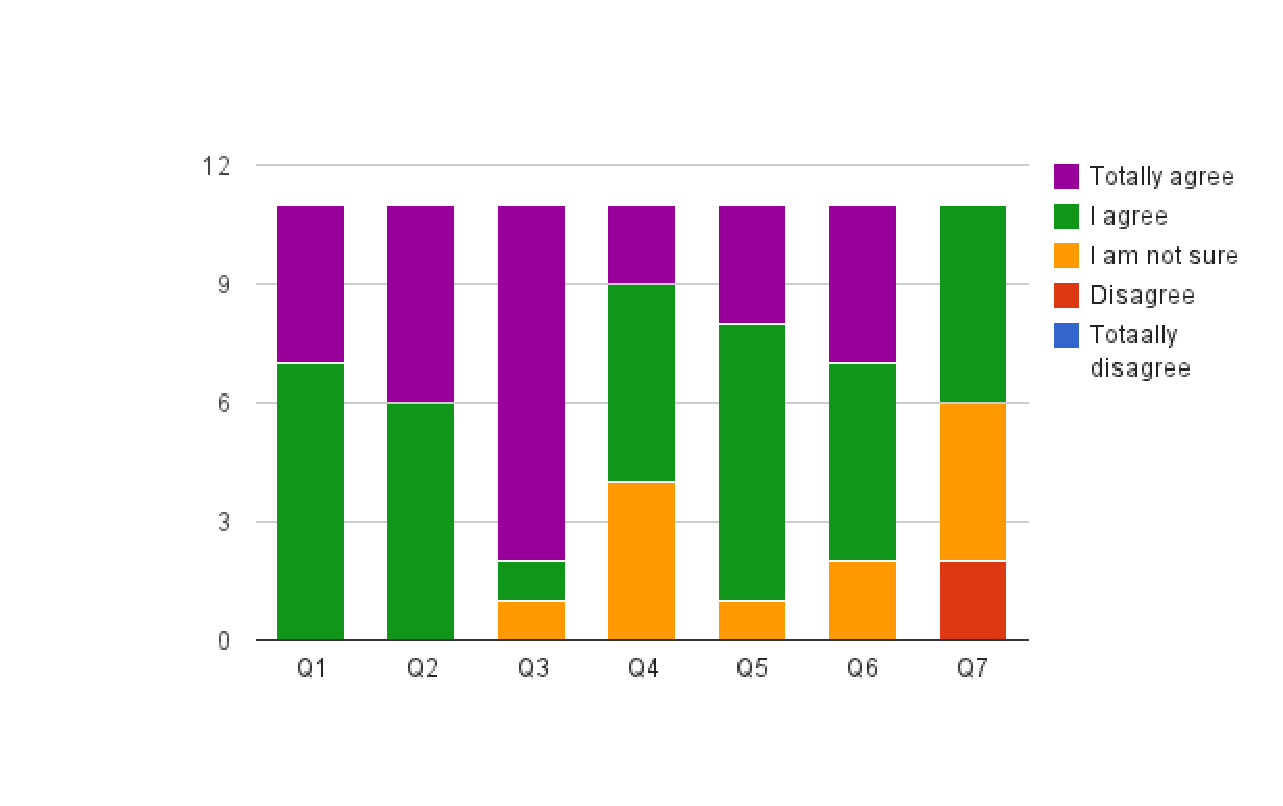
\includegraphics[width=\textwidth]{gfx/agreement.eps}
  \caption{Responses to the questions in Table~\ref{fig:questions2-pgce}} 
\label{fig:additional}
\end{figure}

Figure~\ref{fig:additional} presents the responses relating to each
question. We see that there are no responses of Totally Disagree to any question,
and that only Q7 attracted 2 answers of Disagree. Q1, Q2, Q3, Q5, Q6
had mostly responses of Agree or Totally Agree. Q4 had 4 responses of
Not Sure, and it related to using the tools to inform the provision of
support and guidance to students during the lesson. Q7 had the worst
pattern of responses, with 2 answers of Disagree and 4 answers of Not
Sure, and it related to identifying common conceptual or procedural
difficulties that students are facing. We discuss these results in
more detail in the next Section.




%%% Local Variables:
%%% mode: latex
%%% TeX-master: "main"
%%% End:
